\documentclass[article, table, xcdraw]{article}

\usepackage{bbm}
\usepackage{amsmath}
\usepackage{mathtools}
\usepackage{empheq}
\usepackage[italian]{babel}
\usepackage[utf8]{inputenc}
\usepackage{physics}
\usepackage{multirow}
\usepackage{xifthen}
\usepackage[table,xcdraw]{xcolor}
\usepackage{tkz-graph}
\usepackage{listings}
\usepackage{color}
\usepackage{graphicx}
\usepackage{framed}

\title{Calcolo Numerico - die Beziehung}
\date{10 giugno 2018}
\author{Saftoiu Vlad Alexandru}

\definecolor{shadecolor}{rgb}{1,1,0.5}
\definecolor{dkgreen}{rgb}{0,0.6,0}
\definecolor{gray}{rgb}{0.5,0.5,0.5}
\definecolor{mauve}{rgb}{0.58,0,0.82}

\DeclarePairedDelimiter{\ceil}{\lceil}{\rceil}

\lstset{frame=tb,
  language=Matlab,
  aboveskip=3mm,
  belowskip=3mm,
  showstringspaces=false,
  columns=flexible,
  basicstyle={\small\ttfamily},
  numbers=none,
  numberstyle=\tiny\color{gray},
  keywordstyle=\color{blue},
  commentstyle=\color{dkgreen},
  stringstyle=\color{mauve},
  breaklines=true,
  breakatwhitespace=true,
  tabsize=3
}


\begin{document}
	
	\newcommand{\TODO}[1][]{
		\begin{shaded*} 
			da fare \ifthenelse{\isempty{#1}}{ }{ (: #1 ) }
		\end{shaded*}
	}
	
	\newcommand{\fek}[1]{
		\begin{equation*}
			#1
		\end{equation*}
	}

	\newcommand{\PP}[1][]{
		\ifthenelse{ \isempty{#1} }{ \\[10pt] }{ \\[#1pt] }
	}

	\pagenumbering{gobble}
	\maketitle
	\newpage
	\pagenumbering{arabic}

	\tableofcontents
	\newpage
	
	\section{Capitolo 1}


	\subsection{Esercizio 1.1}

Sia $x = e \approx 2.7183 = \tilde{x}$. Si calcoli il corrispondente errore relativo $\varepsilon_x$ e il numero di cifre significative $k$ con cui $\tilde{x}$ approssima $x$. Si verifichi che:

\fek{\abs{\varepsilon_x} \approx \frac{1}{2}10^{-k}}

L'errore relativo è la quantità: $\varepsilon_x \equiv \frac{\Delta{x}}{x}=\frac{\tilde{x}-x}{x} = \frac{2.7183-e}{e} = 6.68494 \times 10^{-6}$.\\
Il numero di cifre significative $k$ è all'incirca $-\log_{10}{\abs{\varepsilon_x}}$ ovvero: 
\fek{-\log_{10}{6.68494 \times 10^{-6}}=5.174 \approx 5}.\\
Infatti le prime 5 cifre decimali dell'approssimazione $\tilde{x}$ sono corrette: $\tilde{x}  =\underline{2.7183}$ e $x = \underline{2.71828}182845...$.\\
Inoltre si verifica che: $\abs{\varepsilon_x} = \abs{6.685 \times 10^{-6}} = 0.6685 \times 10^{-5} \approx \frac{1}{2}10^{-5}$


	\subsection{Esercizio 1.2}
	
	Usando gli sviluppi di Taylor fino al secondo ordine con resto in forma di Lagrange, si verifiche che se $f \in C^3$, risulta:
	
\fek{f^{(1)}(x) = \phi_h(x) + O(h^2)}

	dove

\fek{\phi_h(x) = \frac{f(x+h)-f(x-h)}{2h}}

Sapendo che lo sviluppo del polinomio di Taylor al secondo ordine, centrato in un punto $x_0$ è:
\fek{ f(x) = f(x_0) + (x -x_0) f^{(1)}(x_0)+\frac{(x-x_0)^2}{2}f^{(2)}(x_0) +O((x-x_0)^3) }
si ha che:
\begin{equation*}
	\begin{split}
	f(x+h) & = f(x_0) + hf^{(1)}(x_0)+\frac{h^2}{2}f^{(2)}(x_0) + O(h^3) \\
	f(x-h) & = f(x_0) - hf^{(1)}(x_0)+\frac{h^2}{2}f^{(2)}(x_0) + O(h^3) \\	
	\end{split}
\end{equation*}
Sostituendo lo sviluppo a $f(x \pm h)$ si ottiene:
\begin{equation*}
	\begin{split}
\frac{f(x_0) + hf^{(1)}(x_0)+\frac{h^2}{2}f^{(2)}(x_0) + O(h^3) - f(x_0) + hf^{(1)}(x_0)-\frac{h^2}{2}f^{(2)}(x_0) + O(h^3)}{2h}\\ 
	= \frac{2hf^{(1)}(x_0) + O(h^3)}{2h} = f^{(1)}(x_0) + O(h^2)
	\end{split}
\end{equation*}


	\subsection{Esercizio 1.3}
	
Utilizzando Matlab, si costruisca una tabella dove, per $h = 10^{-j}$, $j =1, . . . , 10$ e per la funzione $f(x) = x^{4}$ si riporta il valore di $\phi_h(x)$ definito nell'Esercizio 1 in $x = 1$. Commentare i risultati ottenuti.

Utilizzando lo script:
\lstinputlisting{./capitolo_1/esercizio_3.m}
si ottengono i seguenti risultati:
\begin{tabular}{ c | c }
i & $\phi_h(1)$ \\
\hline
1  & 4.040000000000002e+00 \\
2  & 4.000400000000004e+00 \\
3  & 4.000003999999723e+00 \\
4  & 4.000000039999230e+00 \\
5  & 4.000000000403681e+00 \\
6  & 3.999999999948489e+00 \\
7  & 4.000000000115023e+00 \\
8  & 4.000000003445692e+00 \\
9  & 4.000000108916879e+00 \\
10 & 4.000000330961484e+00 \\
\end{tabular}

	\subsection{Esercizio 1.4}
	
Si dia una maggiorazione del valore assoluto dell’errore relativo con cui $x + y + z$ viene approssimato dall’approssimazione prodotta dal calcolatore, ossia $(x \oplus y) \oplus z$ (supporre che non ci siano problemi di overflow o di underflow). Ricavare l’analoga maggiorazione anche per $x \oplus (y \oplus z)$ tenendo presente che $x \oplus (y \oplus z) = (y \oplus z) \oplus x$.

Tenendo presente la funzione $fl: \mathrm{I} \rightarrow \mathrm{M}$ definita come: $fl(x) \equiv \tilde{x} = x(1+\varepsilon_x)$ e considerando che in aritmentica esatta $(x+y)+z = x+y+z$, l'errore relativo è misurato come $\frac{\tilde{x}-x}{x} = \frac{(x \oplus y) \oplus z - x - y - z}{x+y+z}$ e quindi si ha:
\begin{equation*}
	\begin{split}
		(x \oplus y) \oplus z \\
			& = fl \lbrack \; fl(fl(x) + fl(y)) + fl(z) \;\rbrack \\
			& = fl \lbrack \; fl(x(1+\varepsilon_x) + y(1+\varepsilon_y)) + z(1+\varepsilon_z) \; \rbrack \\
			& = fl \{ \; \lbrack \; x(1+\varepsilon_x) + y(1+\varepsilon_y) \; \rbrack (1 + \varepsilon_{\alpha}) + z(1+\varepsilon_z) \; \} \\
	  		& = \{ \; \lbrack \; x(1+\varepsilon_x) + y(1+\varepsilon_y) \; \rbrack (1 + \varepsilon_{\alpha}) + z(1+\varepsilon_z) \; \} (1 + \varepsilon_{\beta}) \\
	\end{split}
\end{equation*}

\begin{equation*}
	\begin{split}
		\frac{(x \oplus y) \oplus z - x - y - z}{x+y+z} \\
			& \leq \frac{x(1+u)^3 + y(1+u)^2 + z(1+u^2) -x -y -z}{x+y+z} \\
	 		& = \frac{x(3u+3u^2+u^3) + y(3u+3u^2+u^3) + z(2u+u^2)}{x+y+z} \\
	 		& \leq \frac{x(3u+3u^2+u^3) + y(3u+3u^2+u^3) + z(2u+u^2)}{x+y+z} \\
	 		& \leq \frac{7ux+7uy+3uz}{x+y+z} \\
	 		& = u(3+4 \frac{x+y}{x+y+z})
	\end{split}
\end{equation*}


	\subsection{Esercizio 1.5}
Eseguire le seguenti istruzioni in Matlab:
\begin{lstlisting}[frame=single]
	x = 0; count = 0;	
	while x \tilde= 1, x = x + delta, count = count + 1, end
\end{lstlisting}
dapprima ponendo $delta = 1/16$ e poi ponendo $delta = 1/20$. Commentare i risultati ottenuti e in particolare il non funzionamento nel secondo caso.
\par
Il numero $1/16 = 0.0625$ in binario è: $0.0001$\\
Invece il numero $1/20 = 0.05$ in binario risulta periodico: $0.00\underline{0011}$, questo significa che, memorizzandolo in un area di memoria finita, si ha necessariamente perdita di informazione; in particolare:\\
IEEE 754 (base 2): $00111101010011001100110011001101$\\
ovvero in base 10: $0.0500000007450580596923828125 > 0.05$\\
pertanto $\phi_{20} = 1.0000000149 \neq 1$ e quindi il ciclo non concluderà mai.

	\subsection{Esercizio 1.6}
Verificare che entrambe le seguenti successioni convergono a $\sqrt{3}$ , (riportare le successive approssimazioni in una tabella a due colonne, una per ciascuna successione),
\fek{x_{k+1} = \frac{x_k + \frac{3}{x_k}}{2}, \quad x_0 = 3}
\fek{x_{k+1} = \frac{3+x_{k-1}x_k}{x_{k-1}+x_k}, \quad x_0 = 3, x_1=2}
Per ciascuna delle due successioni, dire quindi dopo quante iterazioni si ottiene un’approssimazione con un errore assoluto minore o uguale a $10^{-12}$ in valore assoluto.

\par
Usando lo script:
\lstinputlisting{./capitolo_1/esercizio_6.m}
si ottengono i seguenti risultati:

\begin{tabular}{ r | c | c | c | c }
		
  \textbf{i} & \textbf{$s_1$} & \textbf{$e_1$} & \textbf{$s_2$} & \textbf{$e_2$} \\
  \hline	
  	1 & 3.0000000 &                & 3.0000000 &               \\
	2 & 2.0000000 & 2.6794919 e-01 & 2.0000000 &               \\
	3 & 1.7500000 & 1.7949192 e-02 & 1.8000000 & 6.7949192 e-02\\
	4 & 1.7321429 & 9.2049574 e-05 & 1.7368420 & 4.7912977 e-03\\
	5 & 1.7320508 & 2.4458502 e-09 & 1.7321429 & 9.2049574 e-05\\
	6 & 1.7320508 &                & 1.7320509 & 1.2713716 e-07\\
	7 &           &                & 1.7320508 & 3.3786307 e-12\\
	8 &           &                & 1.7320508 & 2.2204460 e-16\\
  \hline  
\end{tabular}

Si verifica che entrambe le successioni convergono al valore $\sqrt{3}$, la prima successione converge più velocemente e l'errore assoluto sarà minore o uguale a $10^{-12}$ dopo la 5a iterazione, mentre per la seconda successione questo avviene dopo la 7a iterazione.
	\section{Capitolo 4}
	\subsection{Comunicazione su canali rumorosi}
	L'argomento della comunicazione affidabile tramite canali rumorosi è stata trattata in maniera approfondita da Claude E. Shannon, in particolare è di grande importanza l'omonimo teorema \textit{Shannon's coding theorem} che collega la capacità di un canale \textit{Ch} al rate di trasmissione dell'informazione, ovvero al rapporto $\frac{K}{N}$ tra i $K$ bit di informazione utile e l'utilizzo del canale (numero di bit trasmessi $N$). In particolare è verificato che per un $N$ \textit{sufficientemente} grande è possibile circoscrivere la probabilità di errore entro un arbitrario $\varepsilon$ fissato. Tuttavia aumentando la dimensione $N$ dei blocchi si ha anche, nel caso di codici a blocchi non sparsi, un aumento di ordine quadratico del numero di nodi del grafo associato alla matrice di parity check, che comporta un notevole impiego di risorse durante la fase di decodifica.
	\subsection {Low Density Parity Check codes}
	I \textit{LDPC} sono una classe di codici lineari introdotta per la prima volta da Robert G. Gallager negli anni 1960 che permettono di raggiungere un \textit{rate} di trasmissione delle informazioni tramite un canale rumoroso molto buone aumentando la dimensione dei blocchi senza pesare eccessivamente sull'algoritmo di decodifica.
	
	Un codice \textit{LDPC} è un codice a blocchi con una matriche di controllo $\textbf{H}$ sparsa ovvero con "pochi" uno su ogni riga e su ogni colonna (il numero dei checks può addirittura rimanere invariato al crescere di N). Un codice a blocchi è regolare quando, data una matrice $\textbf{H} \in M_{m \times n}$ con elementi in $\left\{0,1\right\}$ si ha che:
	\begin{equation}
		\forall i = 1 ... m \quad W_{ham}(\textbf{H}_i) = K
	\end{equation}
	\begin{equation}
		  \forall j =1 ... n \quad W_{ham}(\textbf{H}^j) = J 
	\end{equation}
	
	La famiglia dei codici LDPC ha una buona distanza $d$, ovvero il rapporto $d/N$ tende a una costante maggiore di zero, considerando $N$ come lunghezza del blocco. Il problema è riuscire a costruire un decoder efficiente che, dato l'output $\textbf{r}$ sul canale C, individua la codeword $\textbf{t}$ con la probabilità $P(\textbf{r}|\textbf{t})$ maggiore. 

Decodificare un codice LDPC è un problema NP-completo, un approccio che possiamo seguire per ottenere un decoder è dato dall'utilizzo dell'algoritmo somme-prodotti a scambio di messaggi.

	Le caratteristiche principali dei codici LDPC sono: 
	\begin{itemize}
		\item si possono implementare per un N arbitrario;
		\item la complessità legata alla decodifica è relativamente bassa;
		\item sono di facile implementazione;
		\item c'è un buon rapporto errori / blocco.
	\end{itemize}
	\section{Capitolo 3}


	\subsection{Esercizio 3.1}

Scrivere una function Matlab per la risoluzione di un sistema lineare con matrice dei coefficienti triangolare inferiore a diagonale unitaria. Inserire un esempio di utilizzo.

La function per risolvere il sistema su indicato è la seguente:

\lstinputlisting{./capitolo_3/solve_t_inf_udiag.m}

che viene utilizzata passando la matrice $A$ e il vettore dei termini noti $\mathbf{b}$ che verrà sovrascritto con il vettore $\mathbf{x}$ via via calcolato dentro la function. 
Un esempio di utilizzo, per risolvere il sistema $A\mathbf{x}=\mathbf{b}$ con
	\[	
		A = 
		\begin{pmatrix}
			1&0&0&0&0 \\
			3&1&0&0&0\\
			-1&2&1&0&0\\
			2&-4&-2&1&0\\
			3&3&1&3&1\\
		\end{pmatrix}
	\]
	\[  
		\mathbf{b}=(4,-5,-38,77,-40)
	\]
	
 è il seguente:
 
\lstinputlisting{./capitolo_3/solve_t_inf_udiag_test.m}

il risultato è il seguente (compresa verifica moltiplicando per la matrice iniziale):

\begin{lstlisting}[frame=single]

>> solve_t_inf_udiag_test

x =    4   -17     0     1    -4

ans =     0     0     0     0     0

\end{lstlisting}

	\subsection{Esercizio 3.2}

Utilizzare l'algoritmo 3.6 del libro per stabilire se le seguenti matrici sono $sdp$ o no:
	\[	
		A_1 = 
		\begin{pmatrix}
			1&-1&2&2 \\
			-1&5&-14&2\\
			2&-14&42&2\\
			2&2&2&65\\
		\end{pmatrix}
	\]
	\[		
		A_2 =
		\begin{pmatrix}
			1&-1&2&2\\
			-1&6&-17&3\\
			2&-17&48&-16\\
			2&3&-16&4\\
		\end{pmatrix}
	\]

Usando lo script: \\
\lstinputlisting{./capitolo_1/sdp_test.m}
che si appoggia all'algoritmo 3.6:\\
\lstinputlisting{./capitolo_3/LDL.m}
I risultati sono i seguenti:\\
\begin{lstlisting}[frame=single]
sdp_test

A =

     1    -1     2     2
    -1     5   -14     2
     2   -14    42     2
     2     2     2    65

la matrice e' SDP

A =

     1    -1     2     2
    -1     6   -17     3
     2   -17    48   -16
     2     3   -16     4

la matrice NON e' SDP
\end{lstlisting}


	\subsection{Esercizio 3.3}

Scrivere una function Matlab che, avendo in ingresso un vettore $b$ contenente i termini noti del sistema lineare $Ax = b$ con $A$ sdp e l’output dell’Algoritmo 3.6 del libro (matrice $A$ riscritta nella porzione triangolare inferiore con i fattori $L$ e $D$ della fattorizzazione $LDL^{T}$ di $A$), ne calcoli efficientemente la soluzione.

\lstinputlisting{./capitolo_3/solve_with_ldl.m}



	\subsection{Esercizio 3.4}

Scrivere una function Matlab che, avendo in ingresso un vettore $b$ contenente i termini noti del sistema lineare $Ax = b$ e l’output dell’Algoritmo 3.7 del libro (matrice $A$ riscritta con la fattorizzazione $LU$ con pivoting parziale e il vettore $p$ delle permutazioni), ne calcoli efficientemente la soluzione.

\lstinputlisting{./capitolo_3/solve_with_lu_pivoting.m}


	\subsection{Esercizio 3.5}

 Inserire alcuni esempi di utilizzo delle due function implementate per i punti 3 e 4, scegliendo per ciascuno di essi un vettore $\tilde{x}$ e ponendo $b = A\tilde{x}$. Riportare $\tilde{x}$ e la soluzione $x$ da essi prodotta. Costruire anche una tabella in cui, per ogni esempio considerato, si riportano il numero di condizionamento di $A$ in norma 2 (usare $cond$ di Matlab) e le quantità $\frac{\norm{r}}{\norm{b}}$ e $\frac{\norm{x-\tilde{x}}}{\norm{\tilde{x}}}$.

Utilizzando lo script:

\lstinputlisting{./capitolo_3/exercise_5.m}

si verifica che....
\TODO[inserire tabella carina con risultati dello script e considerazioni]


	\subsection{Esercizio 3.6}

Sia $A = \begin{pmatrix} \epsilon & 1 \\ 1 & 1  \end{pmatrix}$ con $\epsilon = 10^{-13}$. Definire $L$ triangolare inferiore a diagonale unitaria e $U$ triangolare superiore in modo che il prodotto $LU$ sia la fattorizzazione $LU$ di $A$ e, posto $\mathbf{b} = A\mathbf{e}$, con $\mathbf{e} = (1, 1)^T$, confrontare l'accuratezza della soluzione che si ottiene usando il comando $U\setminus(L\setminus \mathbf{b})$ (Gauss senza pivoting) e il comando $A\setminus \mathbf{b}$ (Gauss con pivoting).

Una fattorizzazione $LU$ di A è: $L = \begin{pmatrix} 1 & 0 \\ \frac{1}{\epsilon} & 1  \end{pmatrix}, U = \begin{pmatrix} \epsilon & 1 \\ 0 & -\epsilon  \end{pmatrix}$, tuttavia eseguendo $U\setminus(L\setminus \mathbf{b})$ si ottiene $\mathbf{x} = (0.999200722162641, 1.000000000000000)^T$ ed un warning: `\textit{Matrix is close to singular or badly scaled. Results may be inaccurate. RCOND =
1.000000e-26}`. Infatti si verifica subito che numero di condizionamento delle matrici L ed U non sono buoni: entrambi sono dell'ordine di $e+25$.
Lo script usato per questo esercizio è:
\lstinputlisting{./capitolo_3/exercise_6.m}


	\subsection{Esercizio 3.7}
Scrivere una function Matlab specifica per la risoluzione di un sistema lineare con matrice dei coefficienti $A \in \mathcal{R}^{n \times n}$ bidiagonale inferiore a diagonale unitaria di Toeplitz, specificabile con uno scalare $\alpha$. Sperimentarne e commentarne le prestazioni (considerare il numero di condizionamento della matrice) nel caso in cui $n = 12$ e $\alpha =100$ ponendo dapprima $b = (1, 101, \dots , 101)^T$ (soluzione esatta $\tilde{x} = (1, \dots , 1)^T$ ) e quindi $b = 0.1 * (1, 101, \dots , 101)^T$ (soluzione esatta $\tilde{x} = (0.1, \dots , 0.1)^T$).

La funzione per risolvere una matrice bidiagonale inferiore di Toeplitz è la seguente:
\lstinputlisting{./capitolo_3/solve_bidiagonal_toeplitz.m}
Dato che la matrice bidiagonale inferiore di T. è (se non ho capito male) della forma:
\[
\begin{pmatrix}
	1&0&0&0&0\\
	\alpha&1&0&0&0\\
	0&\alpha&1&0&0\\
	0&0&\alpha&1&0\\
	0&0&0&\alpha&1\\
\end{pmatrix}
\]
non è necessario passare alla funzione una matrice intera ma soltanto il vettore $\mathbf{b}$ ed il parametro $\alpha$.
La risoluzione del sistema passa quindi per la seguente semplice formula: 
\fek{x_i = b_i-\alpha x_{i-1} \qquad i=2,3...n } 
Nella funzione Matlab è quindi possibile riscrivere direttamente il vettore in ingresso $\mathbf{b}$.
L'algoritmo ha quindi una occupazione di memoria pari alle $n+1$ posizioni di memoria date dal vettore in ingresso $\mathbf{b}$ e dal parametro $\alpha$; riguardo al numero di operazioni ad ogni passo si esegue una sottrazione e una moltiplicazione quindi queste saranno $2(n-1)$ flops.
La funzione è stata testata verificando la $\mathbf{\tilde{x}}$ risultato dell'algoritmo rispetto alla $\mathbf{x} = A\setminus\mathbf{b}$:
\lstinputlisting{./capitolo_3/solve_bidiagonal_toeplitz_test.m}


	\subsection{Esercizio 3.8}
Scrivere una function che, dato un sistema lineare sovradeterminato $A\mathbf{x}=\mathbf{b}$ con $A \in \mathcal{R}^{m \times n}, m > n, rank(A) = n$ e $\mathbf{b} \in \mathcal{R}^m$, preso come input $\mathbf{b}$ e l'output dell'algoritmo 3.8 del libro (matrice $A$ riscritta con la parte significativa di $R$ e la parte significativa dei vettori di Householder normalizzati con prima componente unitaria), ne calcoli efficientemente la soluzione nel senso dei minimi quadrati.

\TODO


 
	\subsection{Esercizio 3.9}
Inserire due esempi di utilizzo della function implementata per il punto 8 e confrontare la soluzione ottenuta con quella fornita dal comando $A\setminus b$.

\TODO


 
	\subsection{Esercizio 3.10}
Scrivere una function che realizza il metodo di Newton per un sistema nonlineare (prevedere un numero massimo di iterazioni e utilizzare il criterio di arresto basato sull’incremento in norma eucliedea). Utilizzare la function costruita al punto 4 per la risoluzione del sistema lineare ad ogni iterazione.

\TODO


 
	\subsection{Esercizio 3.11}
Verificato che la funzione $f(x_1,x_2) = x_1^2 + x_2^3 - x_1x_2$ ha un punto di minimo relativo in $(1/12, 1/6)$, costruire una tabella in cui si riportano il numero di iterazioni eseguite, e la norma eucliedea dell’ultimo incremento e quella dell’ errore con cui viene approssimato il risultato esatto utilizzando la function sviluppata al punto precedente per valori delle tolleranze pari a $10^{-t}$, con $t=3,6$. Utilizzare $(1/2, 1/2)$ come punto di innesco, verificare che la norma dell'errore è molto più piccola di quella dell'incremento (come mai?).

\TODO
	\section{Capitolo 4}



	\subsection{Esercizio 4.1}
	
Scrivere una function Matlab che implementi il calcolo del polinomio interpolante di grado $n$ in forma di Lagrange. La forma della function deve essere del tipo \texttt{ y = lagrange( xi, fi, x ) }.
\PP
La base di Lagrange è così definita:
\begin{equation}
	L_{kn} := \prod_{j=0,j\neq{k}}^n\frac{x-x_j}{x_k-x_j}
\end{equation}
La forma di Lagrange del polinomio interpolante è:
\begin{equation}\label{lagrange_equation}
	\sum_{k=0}^n f(x_k) L_{kn}(x)
\end{equation}
La function Matlab che implementa la \ref{lagrange_equation} è:
\lstinputlisting{./capitolo_4/lagrange.m}
Costi: dati $n$ numero di ascisse di interpolazione e $m$ numero di punti da calcolare l'occupazione di memoria è pari al vettore $\mathbf{y}$ in output che ha dimensione $m$ mentre il numero di flops è $2mn(2n+1)$.



	\subsection {Esercizio 4.2}
	
Scrivere una function Matlab che implementi il calcolo del polinomio interpolante di grado $n$ in forma di Newton. La forma della function deve essere del tipo \texttt{ y = newton( xi, fi, x ) }
\PP
La base di Newton è così definita: 
\begin{empheq}[left=\empheqlbrace]{align}
	& \omega_0(x):=1 \\
	& \omega_1(x):=x-x_0 \\
	& ... \\
	& \omega_{i+1}(x):=(x-x_i)\omega_i(x)
\end{empheq}
La forma di Newton del polinomio interpolante rispetto alla base di Newton è:
\begin{equation} \label{newton_equation}
	\sum_{k=0}^n f[x_0, ... , x_k]\omega_k(x)
\end{equation} 
La function matlab che implementa \ref{newton_equation} è:
\lstinputlisting{./capitolo_4/newton_interpolation.m}



	\subsection {Esercizio 4.3}
	
Scrivere una function Matlab che implementi il calcolo del polinomio interpolante di Hermite. La forma della function deve essere del tipo \texttt{ y = hermite( xi, fi, f1i, x ) }
\PP
Il polinomio interpolante di Hermite richiede un numero pari di ascisse distribuite come segue: 
\begin{equation}
	a <= x_0 < x_{\frac{1}{2}} < x_{1+\frac{1}{2}} < ... < x_n < x_{n+\frac{1}{2}} <= b
\end{equation}
con $\lim{x_{i+\frac{1}{2}} = x_i}$ si ha che $x_0 = x_1$, $x_2=x_3$, etc. Pertanto $f[x_i, x_1]:=f[x_i, x_i]:=f^{(1)}(x_i)$ e l'algoritmo delle differenze divise verrà modificato in modo che al primo passo quando bisogna calcolare $f[x_i, x_i]$ si utilizza il valore della derivata prima che verrà passato come parametro alla funzione.

La function Matlab che implementa il polinomio interpolante di Hermite è:
\lstinputlisting{./capitolo_4/hermite.m}


	\pagebreak
	\subsection {Esercizio 4.4}
	
Utilizzare le functions degli esercizi precedenti per disegnare l'approssimazione della funzione $sin(x)$  nell'intervallo $[0, 2\pi]$, utilizzando le ascisse di interpolazione $x_{i}=i\pi, i=0,1,2$.
\PP
Il codice seguente richiama le funzioni definite in precedenza e disegna un grafico con le funzioni $sin(x)$ ed i polinomi interpolanti.
\lstinputlisting{./capitolo_4/sin_interpolation.m}
Il risultato è stato riportato in figura \ref{sin_interpolation}.

\begin{figure}[h]\label{sin_interpolation}
    \centering
    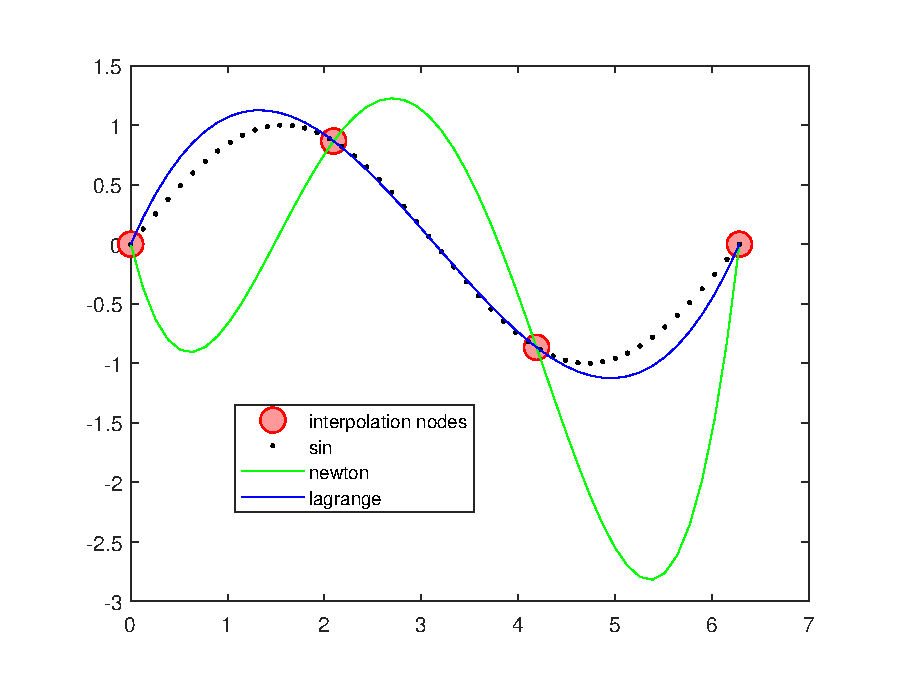
\includegraphics[scale=0.8]{./capitolo_4/sin_interpolation}
    \caption{Interpolazione usando forma di Lagrange e di Newton}
\end{figure} 



	\subsection {Esercizio 4.5}
	
Scrivere una function Matlab che implementi la \texttt { spline } cubica interpolante (naturale o \textit{not-a-knot}, come specificato in ingresso) delle coppie di dati assegnate. La forma della function deve essere del tipo: \texttt { y = spline3( xi, fi, x, tipo ) }.
\PP
Formule per il calcolo della spline cubica:
\begin{equation*}
	\begin{split}
		\forall x \in \lbrack x_{i-1}, x_i \rbrack & : \\
		s_3(x_i) & = \frac{h_i^2}{6}m_i + q_i h_i +r_i \\
		s_3(x_{i-1}) & = \frac{h_i^2}{6}m_{i-1} + r_i \\
		h_i & = x_i - x_{i-1} \\
		q_i & = \frac{f_i - f_{i-1}}{h_i} - \frac{h_i}{6}(m_i -m_{i-1})\\ 
		r_i &= f_{i-1}  - \frac{h_i^2}{6}m_{i-1} \\
		\forall i = 1, 2 \cdots n-1 & : \\
		\varphi_i & = \frac{h_i}{h_i+h_{i+1}} \\
		\xi_i & = \frac{h_{i+1}}{h_i+h_{i+1}} 
	\end{split}
\end{equation*}

I valori $m_i$ sono la soluzione dei seguenti sistemi lineari tridiagonali,
per la spline \textit{naturale}:
\[
	\begin{pmatrix}
		2 		& \xi_1 	& 			& 		& 	\\
		\varphi_2 	& 2			& \xi_2	& 		& 	\\
				& ...			& ...			& ... 	& 	\\
				& 			& ...			& ... 	& \xi_{n-2}	\\
				& 			& 			& \varphi_{n-1} 	& 2	\\
	\end{pmatrix}
	\begin{pmatrix}
		m_1 \\
		m_2 \\
		... \\
		... \\
		m_{n-1}
	\end{pmatrix}
	= 6
	\begin{pmatrix}
		f[x_0, x_1, x_2] \\
		f[x_1, x_2, x_3] \\
		... \\
		... \\
		f[x_{n-2}, x_{n-1}, x_n] \\
	\end{pmatrix}
\]
mentre per la spline \textit{not-a-knot}:
\[
	\begin{smallmatrix}
		1 & 0 & & & & & \\
		\varphi_1 & 2-\varphi_1 & \xi_1 - \varphi_1 & & & & \\
		 & \varphi_2 & 2 & \xi_2 & & & \\
		 & & ... & ... & ... & & \\
		 & & & \varphi_{n-2} & 2 & \xi_{n-2} & \\
		 & & & &  \varphi_{n-1} - \xi_{n-1} & 2-\xi_{n-1} & \xi_{n-1} \\
		 & & & & & 0 & 1 \\
	\end{smallmatrix}
	\begin{smallmatrix}
		m_0+m_1+m_2 \\
		m_1 \\
		... \\
		... \\
		... \\
		m_{n-1}\\
		m_n+m_{n-1}+m_{n-2} \\		
	\end{smallmatrix}
	= 6
	\begin{smallmatrix}
		f[x_0, x_1, x_2] \\
		f[x_0, x_1, x_2] \\
		... \\
		... \\
		... \\
		f[x_{n-2}, x_{n-1}, x_n] \\
		f[x_{n-2}, x_{n-1}, x_n] \\
	\end{smallmatrix}
\]

questo porta al seguente codice per calcolare la spline:
\lstinputlisting{./capitolo_4/my_spline/spline3.m}


	\subsection {Esercizio 4.6}
	
Scrivere una function Matlab che implementi il calcolo delle ascisse di Chebyshev per il polinomio interpolante di grado $n$, su un generico intervallo $[a,b]$. La function deve essere del tipo: \texttt { xi = ceby( n, a, b ) }.
\PP
La function per le ascisse di Chebyshev è:
\lstinputlisting{./capitolo_4/chebyshev_abscissas.m}



	\subsection {Esercizio 4.7}
	
Utilizzare le function degli Esercizi 4.1 e 4.6 per graficare l'approssimazione della funzione di Runge sull'intervallo $[-6,6]$ per $n= 2,4, ... ,40$. Stimare, numericamente, l'errore commesso in funzione del grado $n$ del polinomio interpolante.
\PP
Lo script:
\lstinputlisting{./capitolo_4/exercise_4_7.m}
esegue la function \lstinline{lagrange} con il risultato della function \lstinline{chebyshev_abscissas}, il risultato è stato riportato in figura \ref{4_7_lagrange_interpolation}.\\
\begin{figure}[h!]\label{4_7_lagrange_interpolation}
    \centering
    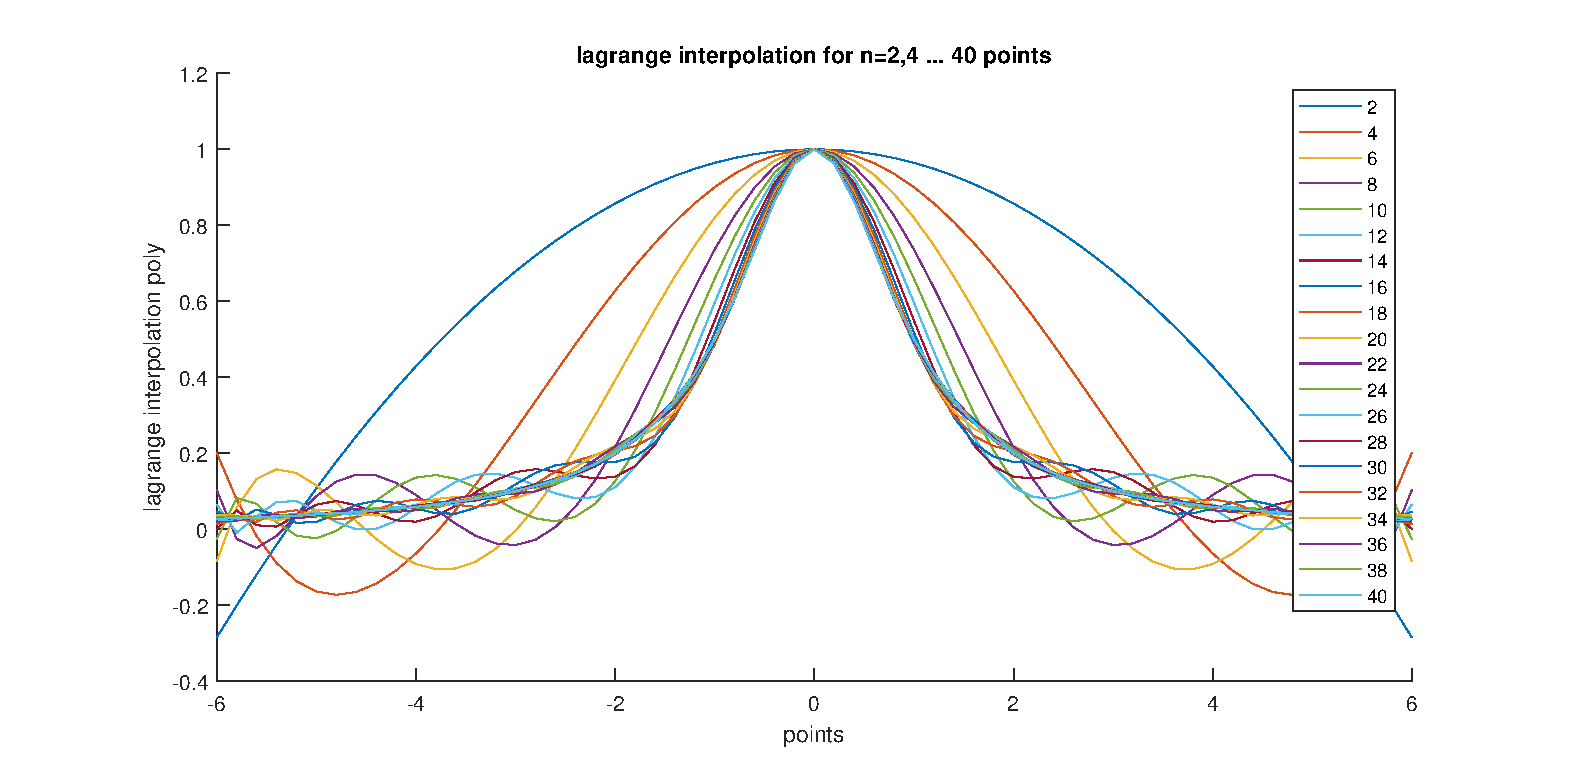
\includegraphics[scale=0.5]{./capitolo_4/exercise_4_7}
    \caption{Interpolazione con ascisse di Chebyshev usando il polinomio in forma di Lagrange per funzione di Runge}
\end{figure}
\PP
L'errore, in relazione al grado $n$ del polinomio, è quantificabile in $\norm{e} <= \frac{\norm{f^{n+1}}}{(n+1)!2^n}$:
\begin{tabular}{ | c | r }
\textbf{n} & \multicolumn{1}{c}{$\mathbf{\norm{e}}$} \\
\hline
2  &   0.18557  \\
4  &  0.051465  \\
6  &  0.013356  \\
8  & 0.0029532  \\
10 & 0.00053885 \\
\end{tabular}
\begin{tabular}{ | c | r }
\textbf{n} & \multicolumn{1}{c}{$\mathbf{\norm{e}}$} \\
\hline
12 & 7.0571e-05 \\
14 & 3.6605e-06 \\
16 & 4.2884e-06 \\
18 &   1.86e-06 \\
20 & 5.7764e-07 \\
\end{tabular}
\begin{tabular}{ | c | r }
\textbf{n} & \multicolumn{1}{c}{$\mathbf{\norm{e}}$} \\
\hline
22 & 1.4887e-07 \\
24 & 3.2687e-08 \\
26 & 5.9039e-09 \\
28 & 7.3124e-10 \\
30 & 3.2957e-11 \\
\end{tabular}
\begin{tabular}{ | c | r }
\textbf{n} & \multicolumn{1}{c}{$\mathbf{\norm{e}}$} \\
\hline
32 & 4.9639e-11 \\
34 & 2.1068e-11 \\
36 & 6.4812e-12 \\
38 & 1.6589e-12 \\
40 & 3.6167e-13
\end{tabular}



	\subsection {Esercizio 4.8}
	
Relativamente al precedente esercizio, stimare numericamente, la crescita della costante di Lebesgue.
\PP
Considerando che la costante di Lebesgue nel caso delle ascisse di Chebyshev è $\Lambda_n \approx \frac{2}{\pi}\log{n} $ si ha la seguente tabella relativa agli $n=2,4,6 ... 40$:\\
\begin{tabular}{ | c | r | r }
\textbf{n} & \multicolumn{1}{c}{$\mathbf{\Lambda_n}$} & \multicolumn{1}{c}{\textbf{\%}}\\
\hline
      2   &  0.44127  &     100  \\
      4   &  0.88254  &     100  \\
      6   &   1.1407  &  29.2  \\
      8   &   1.3238  &  16.0  \\
     10   &   1.4659  &  10.7  \\
\end{tabular}
\begin{tabular}{ | c | r | r }
\textbf{n} & \multicolumn{1}{c}{$\mathbf{\Lambda_n}$} & \multicolumn{1}{c}{\textbf{\%}}\\
\hline
     12   &   1.5819  &  7.9  \\
     14   &   1.6801  &  6.2  \\
     16   &   1.7651  &  5.0  \\
     18   &   1.8401  &  4.2  \\
     20   &   1.9071  &  3.6  \\
\end{tabular}
\begin{tabular}{ | c | r | r }
\textbf{n} & \multicolumn{1}{c}{$\mathbf{\Lambda_n}$} & \multicolumn{1}{c}{\textbf{\%}}\\
\hline
     22   &   1.9678  &  3.1  \\
     24   &   2.0232  &   2.8  \\
     26   &   2.0742  &  2.5  \\
     28   &   2.1213  &  2.3  \\
     30   &   2.1653  &  2.1  \\
\end{tabular}
\begin{tabular}{ | c | r | r }
\textbf{n} & \multicolumn{1}{c}{$\mathbf{\Lambda_n}$} & \multicolumn{1}{c}{\textbf{\%}}\\
\hline
     32   &   2.2064  &  1.9  \\
     34   &    2.245  &  1.7  \\
     36   &   2.2813  &  1.6  \\
     38   &   2.3158  &  1.5  \\
     40   &   2.3484  &  1.4  \\
\end{tabular}



	\subsection {Esercizio 4.9}
	
Utilizzare la function dell'esercizio 4.1 per approssimare la funzione di Runge sull'intervallo $[-6,6]$, su una partizione uniforme di $n+1$ ascisse, $n= 2,4, ... ,40$. Stimare le corrispondenti costanti di Lebesgue.
\PP
Lo script che usa e graficizza il risultato della function \lstinline{lagrange} è il seguente:
\lstinputlisting{./capitolo_4/exercise_4_9.m}
il valore $n$ è stato ristretto a $n=12$ perché oltre la funzione interpolante assume valori elevatissimi in corrispondenza degli estremi ed il grafico non avrebbe nessuna valenza informativa. Già con $n=12$ si verifica che verso gli estremi la funzione assume valori molto elevati e questo è dovuto alla crescita rapida della costante di Lebesgue. 
Il grafico è stato riportato in figura \ref{4_9_lagrange_interpolation}.\\
\begin{figure}[h!]\label{4_9_lagrange_interpolation}
    \centering
    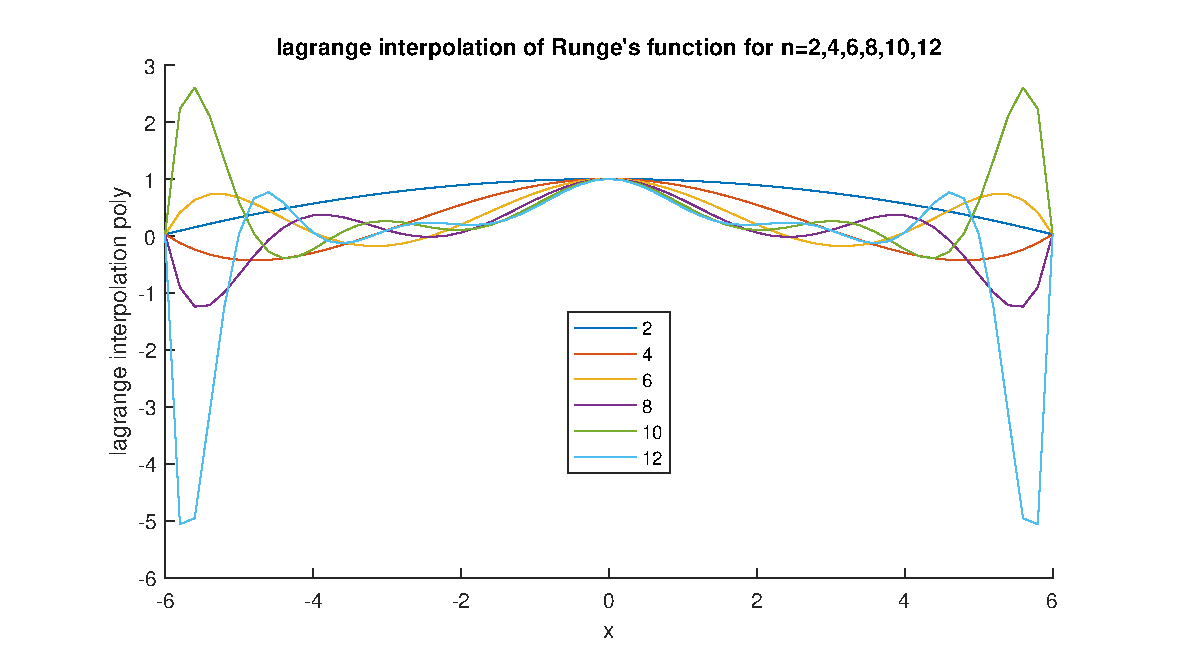
\includegraphics[scale=0.5]{./capitolo_4/exercise_4_9}
    \caption{Interpolazione con ascisse equidistanti usando il polinomio in forma di Lagrange per funzione di Runge}
\end{figure}
Usando questo script:
\lstinputlisting{./capitolo_4/exercise_4_9_lebesgue.m}
anch'esso ristretto a $n=12$ si osserva che la costante aumenta molto rapidamente verso gli estremi all'aumentare di $n$.
Il risultato grafico è riportato in figura \ref{fig:4_9_lebesgue}.\\
\begin{figure}[h!]
    \centering
    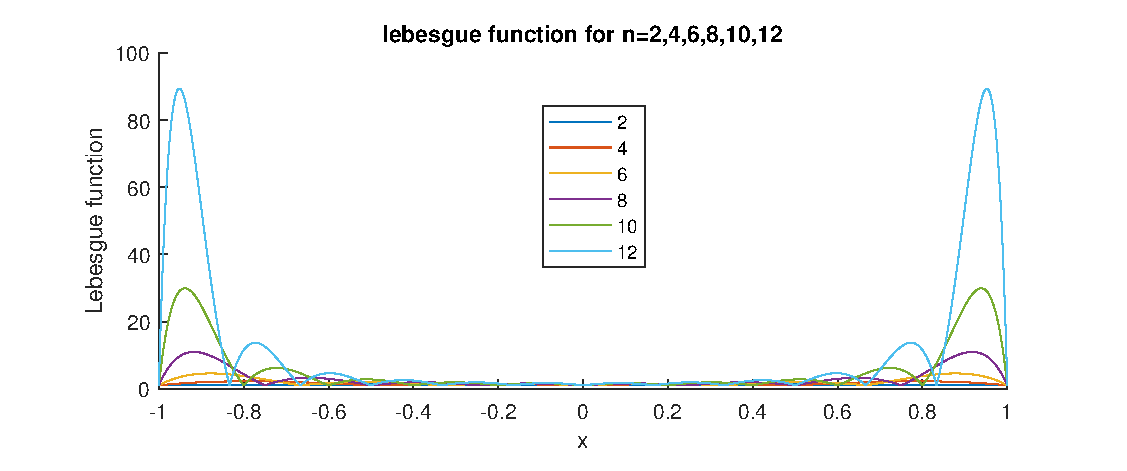
\includegraphics[scale=0.7]{./capitolo_4/exercise_4_9_lebesgue}
    \label{fig:4_9_lebesgue}
    \caption{Valori della funzione di Lebesgue per n= 2,4,6,...,12}
\end{figure}



	\subsection {Esercizio 4.10}

Stimare, nel senso dei minimi quadrati, posizione, velocità iniziale ed accelerazione relative a un moto rettilineao uniformemente accelerato per cui sono note le seguenti misurazioni delle coppie (tempo, spazio): (1, 2.9), (1, 3.1), (2, 6.9), (2, 7.1), (3, 12.9), (3, 13.1), (4, 20.9), (4, 21.1), (5, 30.9), (5, 31.1).
\PP
La formula del moto uniformemente accelerato è:
\begin{equation*}
	x(t) = x_0 + v_0t +\frac{1}/{2}at^2
\end{equation*}
che è un polinomio di grado $n=2$ quindi abbiamo bisogno di almeno $n+1$ ascisse distinte, in questo caso ne abbiamo $5$ pertanto stimare $x_0, \quad v_0, \quad a_0$ equivale a risolvere il seguente sistema sovradeterminato:

\[
	A = 
	\begin{pmatrix}
		1^0 & 1^1 & 1^2 \\
		1^0 & 1^1 & 1^2 \\
		2^0 & 2^1 & 2^2 \\
		2^0 & 2^1 & 2^2 \\
		3^0 & 3^1 & 3^2 \\
		3^0 & 3^1 & 3^2 \\
        	4^0 & 4^1 & 4^2 \\
		4^0 & 4^1 & 4^2 \\
        	5^0 & 5^1 & 5^2 \\
		5^0 & 5^1 & 5^2 \\
	\end{pmatrix}
	\begin{pmatrix}
		x_0 \\
		v_0 \\
		a_0 \\
	\end{pmatrix}
	=
	\begin{pmatrix}
		2.9 \\
		3.1 \\
		6.9 \\
		7.1 \\
		12.9 \\
		13.1 \\
		20.9 \\
		21.1 \\
		30.9 \\
		31.1 \\
	\end{pmatrix}
\]

Usando lo script:

\lstinputlisting{./capitolo_4/exercise_4_10.m}
che risolve il sistema tramite una fattorizzazione $QR$ della matrice $A$ si ottiengono i risultati:
\[
		\mathbf{x} = \begin{pmatrix} x_0 \\ v_0 \\ a_0 \end{pmatrix}  = \begin{pmatrix} 1 \\ 1 \\ 1 \end{pmatrix} 
		, \qquad
		r \equiv A\mathbf{x} - \mathbf{b} = \begin{pmatrix} 0.1 \\ -0.1 \\ 0.1 \\ -0.1 \\ 0.1 \\ -0.1 \\ 0.1 \\ -0.1 \\ 0.1 \\ -0.1 \\ \end{pmatrix} 
\]

	\section{Capitolo 5}

	\subsection{Esercizio 5.1}
Scrivere una function Matlab che implementi la formula composita dei trapezi su $n+1$ ascisse equidistanti nell'intervallo $[a, b]$, relativamente alla funzione implementata da \texttt{fun(x)}. 
La function deve essere del tipo: \texttt{ [If] = trapcomp( n, a, b, fun ) }.
La formula composita dei trapezi è così definita:
\begin{equation}\label{trapezi_composite_equation}
	I_1^{(n)} = \frac{b-a}{2n} (f_0 + 2\sum_{i=1}^{n-1}f_i + f_n)
\end{equation}
La function Matlab che implementa la \ref{trapezi_composite_equation} è:
\lstinputlisting{./capitolo_5/trapcomp.m}


	\section{Capitolo 6}



	\subsection{Esercizio 6.1}
	
Scrivere una function Matlab che generi la matrice sparsa $n \times n$ con $n > 10$, 
$
	A = 
	\begin{pmatrix}
		a_{11} & ... & a_{1n} \\
		. &  & . \\
		a_{n1} & ... & a_{nn}
	\end{pmatrix}
	\quad \text{con} 
$, con $a_{ij} =$ 
\begin{empheq}[left=\empheqlbrace]{align*}
	4,  &  \quad \text{se} \quad i = j \\
	-1, &  \quad \text{se} \quad i = j \pm 1 \\
	-1, &  \quad \text{se} \quad i = j \pm 10 
\end{empheq}
Utilizzare, a questo fine, la function Matlab \lstinline{spdiags}.
\PP
La function che genera la matrice $A$ è la seguente:
\lstinputlisting{./capitolo_6/sparse_diags.m}



	\subsection{Esercizio 6.2}
	
Utilizzare il metodo delle potenze per calcolarne l’autovalore dominante della matrice $A_n$ del precedente esercizio, con una approssimazione $tol = 10^{-5}$, partendo da un vettore con elementi costanti. Riempire, quindi, la seguente
tabella:
\begin{tabular}{|c|c|c|}
\hline
n & numero di iterazioni effettuate & stima autovalore\\
\hline
100 & & \\
200 & & \\
... & & \\
1000 & & \\
\hline
\end{tabular}
\PP
Il metodo delle potenze è implementato dalla seguente function:
\lstinputlisting{./capitolo_6/power_method.m}
la tabella viene generata usando lo script:
\lstinputlisting{./capitolo_6/exercise_6_2.m}
i risultati sono i seguenti:\\
\begin{tabular}{|c|c|r|}
	\hline
	n & iterazioni & stima $\lambda_1 $\\
	\hline
     100   &     46   &    -7.9160  \\
     200   &    103   &     -7.976  \\
     300   &    150   &    -7.9890  \\
     400   &    167   &    -7.9932  \\
     500   &    160   &    -7.9949  \\
	\hline
\end{tabular}
\begin{tabular}{|c|c|r|}
	\hline
	n & iterazioni & stima $\lambda_1 $\\
	\hline
     600   &    154   &    -7.9960  \\
     700   &    132   &    -7.9965  \\
     800   &    123   &    -7.9970  \\
     900   &    115   &    -7.9975  \\
    1000   &    123   &    -7.9975  \\
    	\hline
\end{tabular}



	\subsection{Esercizio 6.3}

Utilizzare il metodo di Jacobi per risolvere il sistema lineare
\begin{equation*}
	A_n \mathbf{x} = \begin{pmatrix} 1 \\ \vdots \\ 1 \end{pmatrix}
\end{equation*}
dove $A_n$ è la matrice definita all'esercizio 6.1, con tolleranza $tol = 10^{-5}$, e partendo dal vettore nullo. Graficare il numero di iterazioni necessarie, rispetto alla dimensione $n$ del problema, con $n$ che varia da $100$ a $1000$ (con passo $20$).
\PP
La function che implementa il metodo di Jacobi è la seguente:
\lstinputlisting{./capitolo_6/jacobi.m}
lo script che la utilizza sugli $n = 100, 120, 140 ... 1000$ è:
\lstinputlisting{./capitolo_6/exercise_6_3.m}
che porta il seguente risultato, rappresentato in figura \ref{fig:6_3_jacobi}.\\
\begin{figure}[h!]
    \centering
    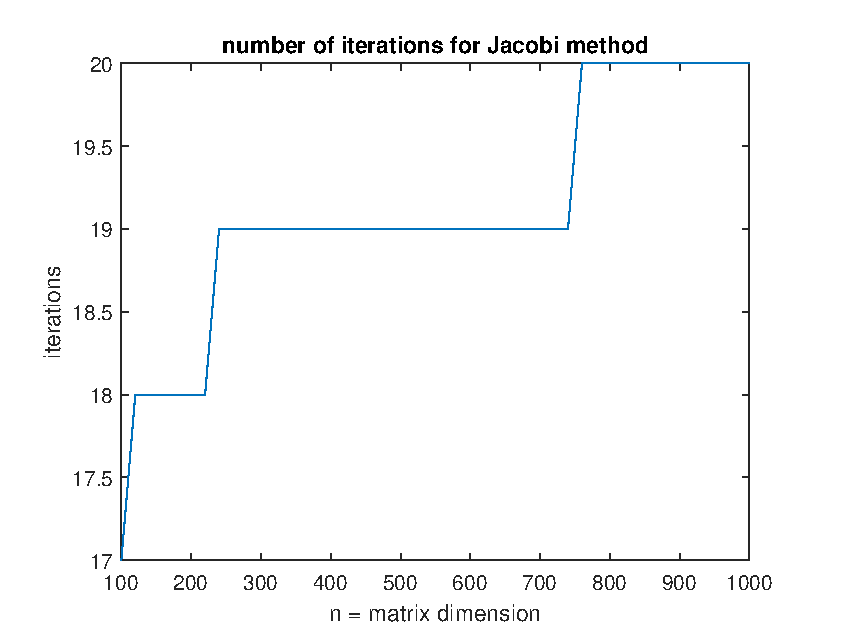
\includegraphics[scale=0.6]{./capitolo_6/exercise_6_3}
    \label{fig:6_3_jacobi}
    \caption{Numero di iterazioni del metodo di Jacobi necessarie per risolvere il sistema per n=100,120...1000}
\end{figure}



	\subsection{Esercizio 6.4}
	
Ripetere una procedura analoga a quella del precedente esercizio utilizzando il medodo di Gauss-Seidel.
\PP
La function che implementa il metodo di Gauss-Seidel è la seguente:
\lstinputlisting{./capitolo_6/gauss_seidel.m}
lo script che la utilizza sugli $n = 100, 120, 140 ... 1000$ è:
\lstinputlisting{./capitolo_6/exercise_6_4.m}
che porta il seguente risultato, rappresentato in figura \ref{fig:6_4_gauss}.\\
\begin{figure}[h!]
    \centering
    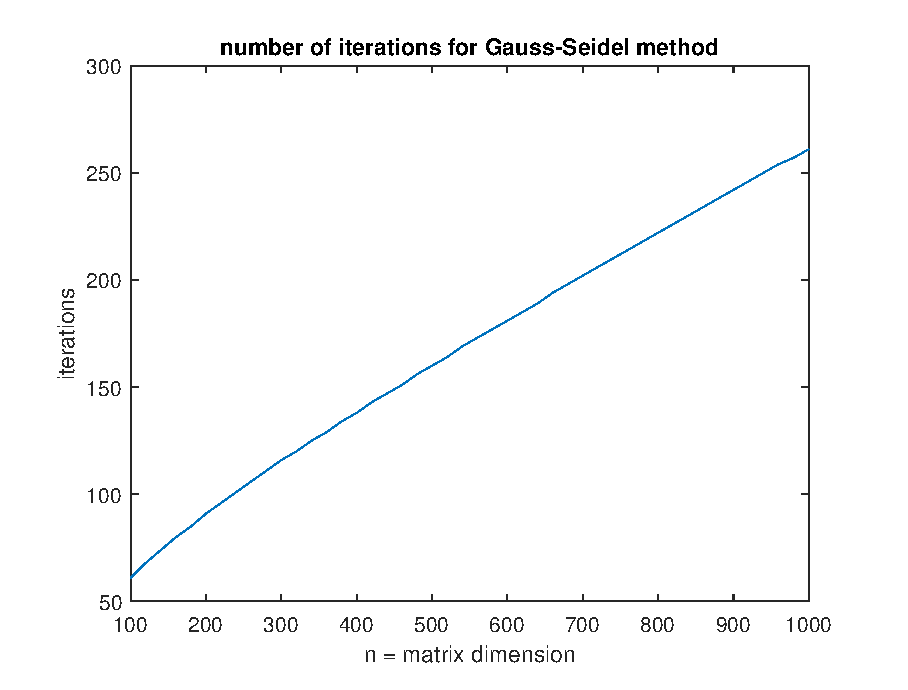
\includegraphics[scale=0.6]{./capitolo_6/exercise_6_4}
    \label{fig:6_4_gauss}
    \caption{Numero di iterazioni del metodo di Gauss-Seidel necessarie per risolvere il sistema per n=100,120...1000}
\end{figure}



	\subsection{Esercizio 6.5}
	
Con riferimento al sistema lineare
\begin{equation*}
	A_n \mathbf{x} = \begin{pmatrix} 1 \\ \vdots \\ 1 \end{pmatrix}
\end{equation*}
con $n = 1000$, graficare la norma dei residui, rispetto all’indice di iterazione, generati dai metodi di Jacobi e GaussSeidel.
Utilizzare il formato \lstinline{semilogy} per realizzare il grafico, corredandolo di opportune \textit{labels}.
\PP
Lo script che utilizza le functions di Jacobi e Gauss-Seidel e ne stampa su un grafico la norma dei residui ad ogni iterazione è il seguente:
\lstinputlisting{./capitolo_6/exercise_6_5.m}
Viene utilizzata una versione leggermente modificata dei due metodi, di cui cambia solo la firma ed il meccanismo interno (con cui ad ogni iterazione, oltre ai calcoli, si memorizza in un vettore $\norm{r}_i$):
\begin{lstlisting}[frame=single]
function [ nrs ] = nrs_gauss_seidel( A, b, tol )
%...

function [ nrs ] = nrs_jacobi( A, b, tol )
%...
\end{lstlisting}

La $\norm{r}$ per iterazione per i due metodi sono rappresentati nelle figure seguenti:
\begin{figure}[h!]
    \centering
    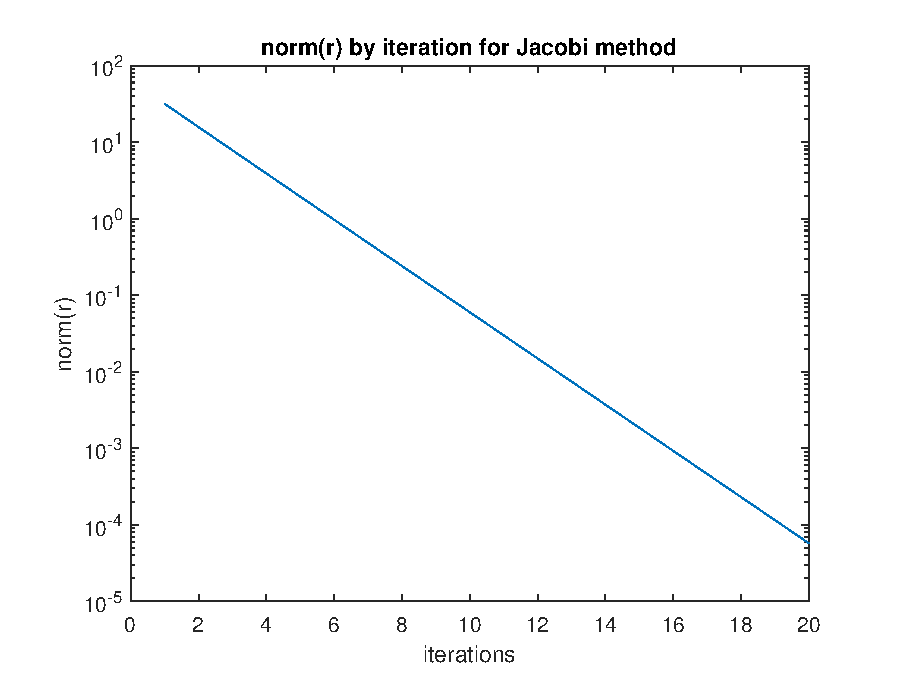
\includegraphics[scale=0.8]{./capitolo_6/exercise_6_5_jacobi}
    \label{fig:6_5_jacobi}
    \caption{$\norm{r}$ per iterazione del metodo di Jacobi}
\end{figure}
\begin{figure}[h!]
    \centering
    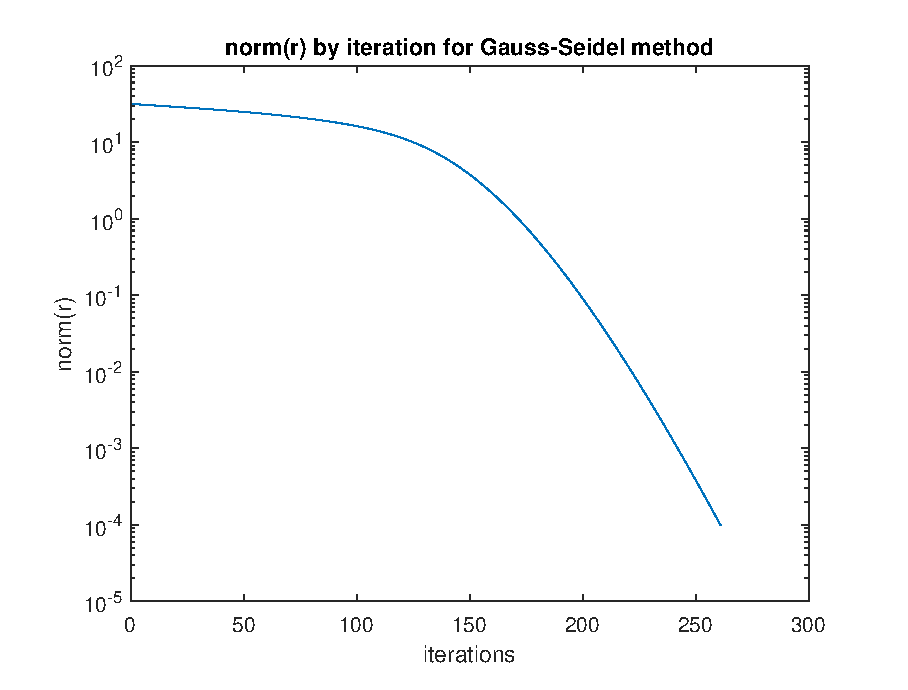
\includegraphics[scale=0.8]{./capitolo_6/exercise_6_5_gauss}
    \label{fig:6_5_gauss}
    \caption{$\norm{r}$ per iterazione del metodo di Gauss-Seidel}
\end{figure}
	
\end{document}